\chapter{Background}
\label{chap:background}

\section{ UML State Diagram}
The Unified Modeling Language\cite{miles_hamilton_2008} (UML) is a standard modeling language for system and software designing and specification. 
It isn't easy to develop a large-scale system.
Too many details can be misinterpreted or forgotten in the development process without some aids. 
Modeling allows us to have a clear vision of the system and capture and communicate with others the essential part of the system. 
So it is quite effective to model a system using the modeling language. 

UML has many types of diagrams. 
Some are static structural, and the rest are dynamic and describe the system's behaviour\cite{UML}. 
The figure shows the hierarchical classification of UML diagrams. 
The version of UML is still being updated and improved today. 
Our concern will only be on the UML state machine diagram, which is dynamic and shows the relations between internal states.
\begin{figure}[ht]
    \centering
    \includegraphics[scale=0.6]{Bilder/UMLOverview.png}
    \caption{The hierarchical classification of UML diagrams\cite{UML}}
    \label{fig:classification}
\end{figure}

UML state machine diagram is also informally called state diagram and in the past is referred to statechart \cite{harel_1987}.
We will illustrate some necessary notations of state diagrams in our current work.

\textbf{State} A state is represented by a rectangle with the state's name in the center. 
If the transition has an effect associated with it, we can also put the effect on the states. 
The diagram represents a state with entry action and exit action.
Actions that occur on events or always occur can also be defined as internal behaviour\cite{state_machine_diagram}.


\begin{figure}[htbp]
\begin{minipage}[t]{0.4\textwidth}
\centering
\includegraphics[width=4cm]{Bilder/sm1.png}
\caption{States\cite{state_machine_diagram}}
\end{minipage}
\begin{minipage}[t]{0.4\textwidth}
\centering
\includegraphics[width=5cm]{Bilder/sm2.png}
\caption{With internal behaviour\cite{state_machine_diagram}}
\end{minipage}
\end{figure}

\textbf{Initial and Final States}
A small filled black circle shows the initial state. 
A circle with a dot inside denotes the final state. 
The initial state should only have outgoing edges.
In contrast, the final state should only have ingoing edges.
\begin{figure}[ht]
    \centering
    \includegraphics[scale=0.55]{Bilder/sm3.png}
    \caption{Initial and Final States\cite{state_machine_diagram}}
    \label{fig:picture4}
\end{figure}

\textbf{History States}
There are two types of history, shallow and deep.
A history state is used to remember the last exited state when interrupted and can be visited after recovery.
\begin{figure}[htbp]
\begin{minipage}[t]{0.4\textwidth}
\centering
\includegraphics[width=1cm]{Bilder/shallow.png}
\caption{Shallow history}
\end{minipage}
\begin{minipage}[t]{0.4\textwidth}
\centering
\includegraphics[width=1cm]{Bilder/deep.png}
\caption{Deep history}
\end{minipage}
\end{figure}

\textbf{Transitions}
A transition in Figure \ref{fig:transitions} is shown with an arrow.
It represents a change of states from the source state to the target state\cite{miles_hamilton_2008}.
In the transition description, there are usually triggers or effects that cause the occurrence of the change.
\begin{figure}[htbp]
\begin{minipage}[t]{0.7\textwidth}
\centering
\includegraphics[width=7.5cm]{Bilder/sm6.png}
\caption{Transitions\cite{state_machine_diagram}}
\label{fig:transitions}
\end{minipage}
\begin{minipage}[t]{0.2\textwidth}
\centering
\includegraphics[width=0.3cm]{Bilder/join.png}
\caption{Fork and join}
\label{fig:fork}
\end{minipage}
\end{figure}

\textbf{Compound States}
There also exist sub-machine diagrams as shown in Figure
\ref{fig:compoundStates}.
\begin{figure}[ht]
    \centering
    \includegraphics[scale=0.4]{Bilder/sm7.png}
    \caption{Compound States\cite{state_machine_diagram}}
    \label{fig:compoundStates}
\end{figure}

\textbf{Fork and Join}
As shown in Figure \ref{fig:fork} and \ref{fig:region}, fork and join are shown as a short thick bar that either branch into concurrent states or rejoin. 
The fork has one ingoing edge and multiple outgoing edges, while the join has multiple ingoing edges and one outgoing edge.

\textbf{Concurrent Regions}
The state can be divided into regions. The exit and execution can occur currently.
\begin{figure}[ht]
    \centering
    \includegraphics[scale=0.55]{Bilder/sm8.png}
    \caption{Concurrent Regions\cite{state_machine_diagram}}
    \label{fig:region}
\end{figure}

\section{ UML State Diagram constructor in Haskell}
\label{sec:UML state Diagram}
In this section, we explain the data type representation of the UML state diagram in Haskell in previous work by Junhao Tan \cite{jun_hao_tan}.
The type constructor \verb|UMLStateDiagram| has six types of data constructors.
And the outermost layer of a state diagram must be a sequential composite diagram.
The \verb|StateDiagram| constructor represents sequential composite states, 
the \verb|CombineDiagram| constructor represents concurrent composite states, 
the \verb|Joint| constructor represents join and fork,
the \verb|History| constructor represents the history node, 
the \verb|InnerMostState| constructor represents the states which contains no substates. 
The \verb|EndState| constructor represents the final states, and the initial states will be defined in \verb|StateDiagram| constructor as \verb|startState|.
   
\begin{verbatim}
type UMLStateDiagram = StateDiagram [Connection]

data StateDiagram a = 
  StateDiagram { substate :: [StateDiagram a],
                    label :: Int,
                    name  :: String,
                    connection :: a,
                    startState :: [Int]
                  }
 | CombineDiagram { substate :: [StateDiagram a],
                    label :: Int
                  }
 | EndState {
     label :: Int
     }
 | Joint { label :: Int
         }
 | History { label :: Int,
             historyType :: HistoryType
           }
 | InnerMostState { label :: Int,
                    name :: String,
                    operations :: String
                  }
deriving (Eq, Functor, Foldable, Show, Traversable)
\end{verbatim}

Each constructor in \verb|UMLStateDiagram| has a label that defines an element uniquely at the same level.
\verb|StateDiagram| has a substate list, a name, a connection list and an integer list that defines the initial state of a state diagram. The connection list lists transitions with a source state, a target state and an action.
For \verb|CombineDiagram|,it has a substate list in which there could only be \verb|StateDiagrams| and at least two \verb|StateDiagrams|.
For \verb|EndState| and \verb|Joint| ,there is no other parameter except the label.
\verb|History| has one parameter called \verb|historyType| which is either \verb|Deep| or \verb|Shallow|.
For \verb|InnerMostState|, it has a name of the state and an optional operations parameter that represents internal behaviours.

Here are some valid instances of state diagram expressions and the corresponding diagrams outputted through our drawing tool.

\begin{verbatim}
picture1 :: UMLStateDiagram
picture1 = StateDiagram [a,b] 1 "" [Connection[1] [2] "t",
           Connection[2] [1,3] ""] []
  where
    a = StateDiagram  [c,d,e] 1 "Composite State" [
        Connection [1] [2] ""] [1]
        where
         c = InnerMostState  1 "State 1" ""
         d = StateDiagram  [f,g] 2 "state 2" [
             Connection [1] [2] ""] [1]
          where
            f = InnerMostState  1 "State 2a" ""
            g = InnerMostState  2 "State 2b" ""
         e = History 3 Deep
    b = InnerMostState  2 "State 3" ""
\end{verbatim}

\begin{figure}[ht]
    \centering
    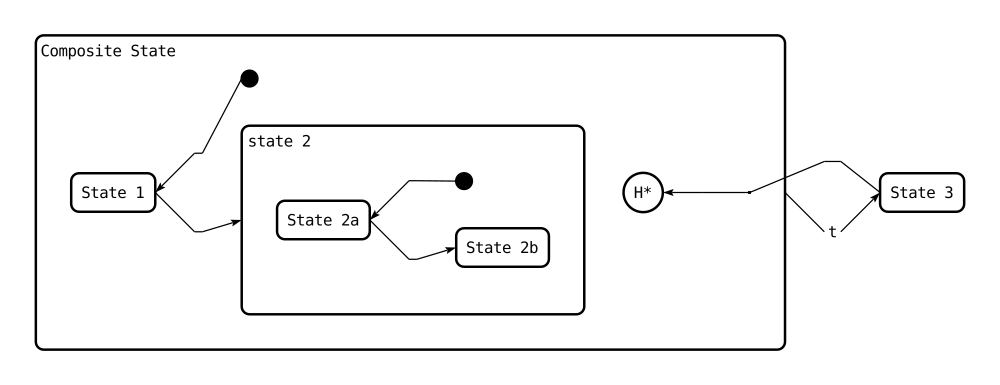
\includegraphics[scale=0.40]{Bilder/picture4.png}
    \caption{picture1}
    \label{fig:picture1}
\end{figure}

\newpage
\begin{verbatim}
picture2 :: UMLStateDiagram
picture2 = StateDiagram [a, b, c, d, l] 1 "" [Connection [1] [2] "a",
           Connection [2, 1, 2] [4] "h", Connection [2, 1, 3] [3] "",
           Connection [2, 2, 2] [3] "", Connection [3] [4] "g",
           Connection [4] [5] ""] [1]
  where
    a = InnerMostState 1 "A" ""
    b = CombineDiagram [e, f] 2
      where
        e = StateDiagram [g, h, i] 1 "" [Connection [1] [2] "b", 
            Connection [2] [3] "c"] [1]
          where
            g = InnerMostState 1 "B" ""
            h = InnerMostState 2 "C" ""
            i = InnerMostState 3 "D" ""
        f = StateDiagram [j, k] 2 "" [Connection [1] [2] "e"] [1]
          where
            j = InnerMostState 1 "E" ""
            k = InnerMostState 2 "F" ""
    c = Joint 3
    d = InnerMostState 4 "G" ""
    l = EndState 5
\end{verbatim}
        
\begin{figure}[ht]
    \centering
    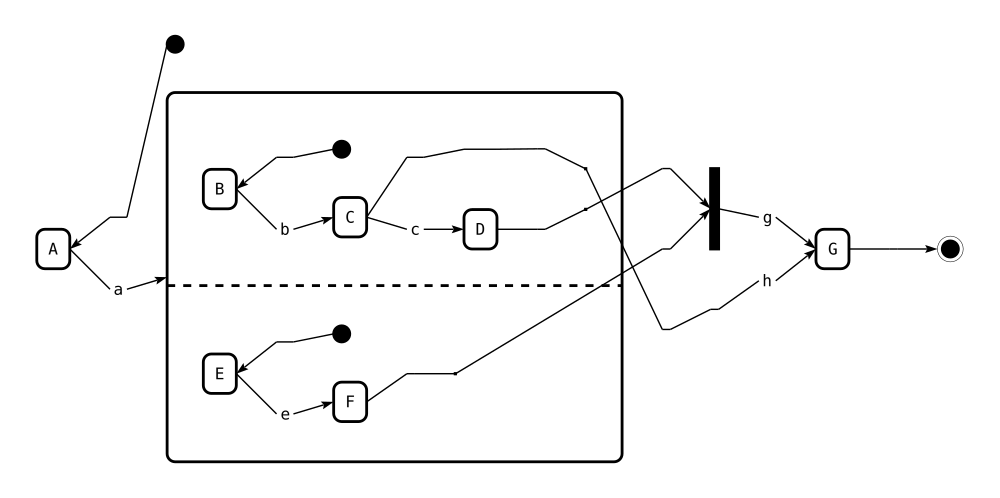
\includegraphics[scale=0.40]{Bilder/slide279.png}
    \caption{picture2}
    \label{fig:picture2}
\end{figure}
In the process of defining properties for a valid expression, we wonder users may input unexpected connections, so we defined two new functions, \verb|localise| and \verb|globalise| in the file of \verb|Datatype|.
Localizing is to transfer connections that are defined globally to local connections. Globalising is to pull all the connections to the outermost layer.
here \verb|[Connection[1,1] [1,2] ""]| is a more global description compared to \verb|[Connection [1] [2] ""]|.
\begin{verbatim}
sample :: UMLStateDiagram
sample = StateDiagram [a,b] 1 "" [Connection[1,1] [1,2] ""] [2]
     wheren
      a = StateDiagram  [c,d] 1 "" [Connection [1] [2] ""] [1]
          where
           c = InnerMostState 1 "A" ""
           d = InnerMostState 2 "B" ""
      b = InnerMostState  2 "C" ""
\end{verbatim}
\newpage

\section{Explanation of existing checkers}
\label{sec:existingCheckers}
Except for the previous presented \verb|UMLStateDiagram| inputs, we still need checkers to ensure that the hand inputs or randomly generated expressions of \verb|UMLStateDiagram| are valid or make sense. 
Hence, we need a thoroughly model-checking tool.
In Jun Hao Tan's thesis \cite{jun_hao_tan}, there already exist two basic checkers called \verb|checkValidity| and \verb|checkWrapper|.

The \verb|checkStructure| limits that none of the diagrams should violate these three properties.
\begin{itemize}
\item  The state machine diagram's outermost layer must be the \verb|StateDiagram|.
\end{itemize}
\begin{itemize}
\item  The \verb|CombineDiagram| constructor must contain at least two \verb|StateDiagram| and no other constructors.
\end{itemize}
\begin{itemize}
\item  The substates of \verb|StateDiagram| constructor cannot be empty or just \verb|History|/ \verb|Joint|.
\end{itemize}

 
The \verb|checkWrapper| defines four properties that must be fulfilled when drawing the diagram:
\begin{itemize}
\item The outermost layer must be the \verb|OrDecom| constructor
\end{itemize}
\begin{itemize}
\item  Substate of \verb|OrDecom| constructor cannot be empty or just \verb|Hist|/ \verb|For|/ \verb|StartS|/ \verb|Dummy|/ \verb|Transition|
\end{itemize}
\begin{itemize}
\item \verb|AndDecom| constructor must contain at least 2 \verb|OrDecom| and no other type of constructor.
\end{itemize}
\begin{itemize}
\item Horizontal slicing must be followed by vertical layering or vise visa
\end{itemize}

Here are counterexamples that the \verb|checkStructure| will reject.

The example \verb|forCheckOuterMostLayer| violates that the outermost layer must be the \verb|StateDiagram|.
Its outer layer is a \verb|CombineDiagram| instead, which is not allowed and will cause a blank \verb|.svg| file while outputting it.

\begin{verbatim}
forCheckOuterMostLayer :: UMLStateDiagram
forCheckOuterMostLayer = CombineDiagram [a,b] 1
     where
        a = StateDiagram  [InnerMostState 1 "A" ""] 1 ""  [] [1]
        b = StateDiagram  [InnerMostState 1 "B" ""] 2 ""  [] [1]
\end{verbatim}

In the \verb|forCheckSubstateSD|, the substrate of \verb|StateDiagram| contains only \verb|History|, violates that the substate of \verb|StateDiagram| constructor cannot be empty or just \verb|History|/ \verb|Joint|.

\begin{verbatim}
forCheckSubstateSD::UMLStateDiagram
forCheckSubstateSD = StateDiagram [a] 1 "" [] [1]
    where
        a = History 1 Deep
\end{verbatim}

Here \verb|forCheckSubstateCD| has only one element \verb|StateDiagram| as substate, violates that the \verb|CombineDiagram| constructor contains at least two \verb|StateDiagrams| and no other constructors.

\begin{verbatim}
forCheckSubstateCD :: UMLStateDiagram
forCheckSubstateCD = StateDiagram [CombineDiagram [a] 1] 1 "" [] []
    where
    a = StateDiagram  [InnerMostState 1 "A" ""] 1 ""  [] [1]
\end{verbatim}


In the further exploring, we split \verb|checkValidity| to two functions \verb|checkRepresatation| and \verb|checkStructure| and add further more testings like verify if outgoing edges from a history node always have the empty transition,the connection points or start points are valid,etc.
We will explain more specifically in a later section \ref{sec:properties}.



\section{ QuickCheck}
\verb|QuickCheck| \cite{claessen_hughes_2000} is a tool used to help programmers formulate and test the properties of programs. 
Properties are defined in Haskell functions and automatically checked on arbitrary inputs.
And a custom-made data generator is also possible to be defined.

If all the randomly generated or hand-input test cases pass the testing, 
it will report "\verb|OK|".
\begin{verbatim}
    +++ OK, passed 100 tests.
\end{verbatim}
Here are some functions we will use in the random inputs generator. 
More detailed examples and information could see \cite{quickcheck}.
\verb|data Gen a| is a generator for values of type \verb|a| \cite{quickcheck}.

If we define a data type of binary tree and do not want to choose a \verb|Leaf| too often,
we can use \verb|frequency| with a reasonale weighted distribution.
Our state diagram datatype could be seen as a tree.
Those states that contain no substates could be \verb|Leaf|.
\begin{verbatim}
    data Tree a = Leaf | Node (Tree a) a (Tree a)
    
    frequency :: [(Int, Gen a)] -> Gen   
\end{verbatim}
\verb|choose| is used to select a random one in the range of two elements.
\begin{verbatim}
    choose :: Random a => (a, a) -> Gen a  
\end{verbatim}
\verb|elements| is similar to \verb|choose|,
but the range of selection could be at arbitrary length but must be non-empty.
\begin{verbatim}
    elements :: [a] -> Gen a 
\end{verbatim}
This function \verb|vectorOf| is used to produce a list of the given length.
\begin{verbatim}
    vectorOf :: Int -> Gen a -> Gen [a]  
\end{verbatim}


